\documentclass[9pt]{beamer}
%------------------------------------------------------------------------
%usepackages
%------------------------------------------------------------------------
\usepackage[utf8]{inputenc}
\usepackage[T1]{fontenc}
\usepackage[utf8]{inputenc}
%!TEX encoding = UTF-8 Unicode
\usefonttheme[onlymath]{serif}
\usepackage{listings}
\usepackage{caption}  
\usepackage{hyperref}
\hypersetup{
    %colorlinks=true,
    %linkcolor=blue,
    %filecolor=magenta,      
    urlcolor=blue,
}
\urlstyle{same}
\usepackage{multicol}
\usepackage{graphics}
\usepackage{standalone}
\usepackage{multimedia}
\usepackage{media9}
\usepackage{graphicx}
\usepackage{empheq}
\usepackage{hyperref}
\hypersetup{
    %colorlinks=true,
    %linkcolor=blue,
    %filecolor=magenta,      
    urlcolor=blue,
    pdftitle={Overleaf Example},
    pdfpagemode=FullScreen,
    }

\usepackage{color}
\usepackage{siunitx}
\usepackage[many]{tcolorbox}
\tcbset{highlight math style={enhanced,
  colframe=red,colback=white,arc=0pt,boxrule=1pt}}
  \tcbset{highlight math style={enhanced,
  colframe=red!60!black,colback=yellow!50!white,arc=4pt,boxrule=1pt,
  drop fuzzy shadow}}
\usepackage{verbatim}
\usepackage{listings}
\usepackage{xcolor}
\definecolor{mygray}{RGB}{245,245,245}
\definecolor{ipython_bg}{RGB}{247, 247, 247}
\definecolor{comentaryGreen}{rgb}{0,0.6,0}
\lstset{
  language=Python,
  numbers=left,
  numberstyle=\footnotesize,
  stepnumber=1,
  columns=fullflexible,
  showspaces=false,
  showstringspaces=false,
  showtabs=false,
  frame=single,
  framerule=0pt,
  basicstyle           = {\normalsize\ttfamily},
  keywordstyle      = \color{blue},
  commentstyle=\color{comentaryGreen},
  stringstyle           = \color{red},
  numberstyle       = \scriptsize\color{gray},
  breaklines=false,
  breakatwhitespace=false,
  escapeinside={\%*}{*)}
}
\usepackage[utf8]{inputenc}
\usetheme{Warsaw}
%\usetheme{Pittsburgh}


%Information to be included in the title page:
\title[Calibration of veto discriminators]{Calibration of veto discriminators}
\subtitle[]{Fragmentation Trigger FOOT}
\author[L. Marini, INFN Pisa ]{L. Marini} 
\institute{INFN Pisa}
\date[October 2021]{October 2021}

\setbeamertemplate{section in toc}{\hspace*{1em}\inserttocsectionnumber.~\inserttocsection\par}
\setbeamertemplate{subsection in toc}{\hspace*{2em}\inserttocsectionnumber.\inserttocsubsectionnumber.~\inserttocsubsection\par}

\begin{document}

\setbeamertemplate{page number in head/foot}[totalframenumber] 
%%%%%%%%%%%%%%%%%%%%%%%%%%%%%%%%%%%%%%%%%%%%%

\frame{\titlepage}


%==================================================================
						%SLIDE - \tableofcontents
%==================================================================

\begin{frame} 
  	\tableofcontents
\end{frame}

%==================================================================
				% SLIDE 
%==================================================================
\section{Calibration}
\subsection{Goal of the measure}
\begin{frame} [fragile]
\small
	\frametitle{Goal of the measure}
	\begin{block}{Goal}
		We want to calibrate the inputs of board wd 166
		 
	\end{block}
	
    	\begin{figure}
	\centering
		\includegraphics[scale=0.3]{figures/crate_configuration/wd166.png}
		
		\caption{FOOT WDAQ crate configuration. Full System}
	\end{figure}  
	
\end{frame}

%==================================================================
				%SLIDE 
%==================================================================
\subsection{Why a calibration?}
\begin{frame} [fragile]
\small
	\frametitle{Why a calibration?}
			
	\begin{alertblock}{Why is calibration necessary?}
		\begin{itemize}
			\item Basically the problem is that the amplitude value [mV] on the PC display and the trigger value are not the same
			\item There is a slight difference between them that needs to be calibrated
			\item A good knowledge of the trigger value is required to be able to trigger between the various fragments
		\end{itemize}
	\end{alertblock}
	    	
		\begin{figure}
		\centering
			\includegraphics[scale=0.17]{photos/why_im.png}
			%\caption{faa.}
		\end{figure}

	
	
\end{frame}




%==================================================================
				%SLIDE 
%==================================================================
\section{Instruments}
\subsection{TGP110 Pulse Generator}
\begin{frame} [fragile]
\small
	\frametitle{TGP110 Pulse Generator}
    		\begin{figure}
		 \centering
			\includegraphics[scale=0.20]{figures/instruments/AIM_TGP110_1k_0.jpg}
			\caption{TGP110. \url{https://resources.aimtti.com/datasheets/AIM-TGP110_pulse_generator_data_sheet-Iss1A.pdf}}
		\end{figure}
\end{frame}

%==================================================================
				%SLIDE 
%==================================================================
\subsection{Crate}
\begin{frame} [fragile]
\small
	\frametitle{Crate}
    		\begin{figure}
		 \centering
			\includegraphics[scale=0.3]{photos/im2.png}
			\caption{Channel 0 to 11 of WaveDream 166.}
		\end{figure}  
\end{frame}


%==================================================================
				%SLIDE 
%==================================================================
\begin{frame} [fragile]
\small
	\frametitle{Connection map TOF}
	
	\colorbox{pink}{Why WaveDream 166?}

\begin{center}
\captionof{table}{X-View TOF.}
\begin{tabular}{ |c|c|c|c|c|c| } 
 	\hline
 	\textbf{Ch TOF} & \textbf{Barra TOF} & \textbf{Nome WD} & \textbf{Slot WD} & \textbf{Ch WD} & \textbf{SiPM}  \\
	 \hline
	 16 & X 8 & \colorbox{green}{wd166} & 6 & 0 & 12 \\ 
	 \hline
	 17 & X 8 & wd166 & 6 & 1 & 50 \\ 
	 \hline
	 18 & X 9 & wd166 & 6 & 2 & 14 \\ 
	 \hline
	 19 & X 9 & wd166 & 6 & 3 & 62 \\ 
	 \hline
	 20 & X 10 & wd166 & 6 & 4 & 15 \\ 
	 \hline
	 21 & X 10 & wd166 & 6 & 5 & 48 \\ 
	 \hline
\end{tabular}
\end{center}

\begin{center}
\captionof{table}{Y-View TOF.}
\begin{tabular}{ |c|c|c|c|c|c| } 
 	\hline
 	\textbf{Ch TOF} & \textbf{Barra TOF} & \textbf{Nome WD} & \textbf{Slot WD} & \textbf{Ch WD} & \textbf{SiPM}  \\
	 \hline
	 56 & Y 8 & wd166 & 6 & 6 & 71 \\ 
	 \hline
	 57 & Y 8 & wd166 & 6 & 7 & 30 \\ 
	 \hline
	 58 & Y 9 & wd166 & 6 & 8 & 65 \\ 
	 \hline
	 59 & Y 9 & wd166 & 6 & 9 & 27 \\ 
	 \hline
	 60 & Y 10 & wd166 & 6 & 10 & 73 \\ 
	 \hline
	 61 & Y 10 & wd166 & 6 & 11 & 25 \\ 
	 \hline
\end{tabular}
\end{center}

\end{frame}

%==================================================================
				%SLIDE 
%==================================================================
\section{Method}
\subsection{Amplitude and Trigger correlation}
\begin{frame} [fragile]
\small
	\frametitle{Method}
    		\begin{figure}
		 \centering
			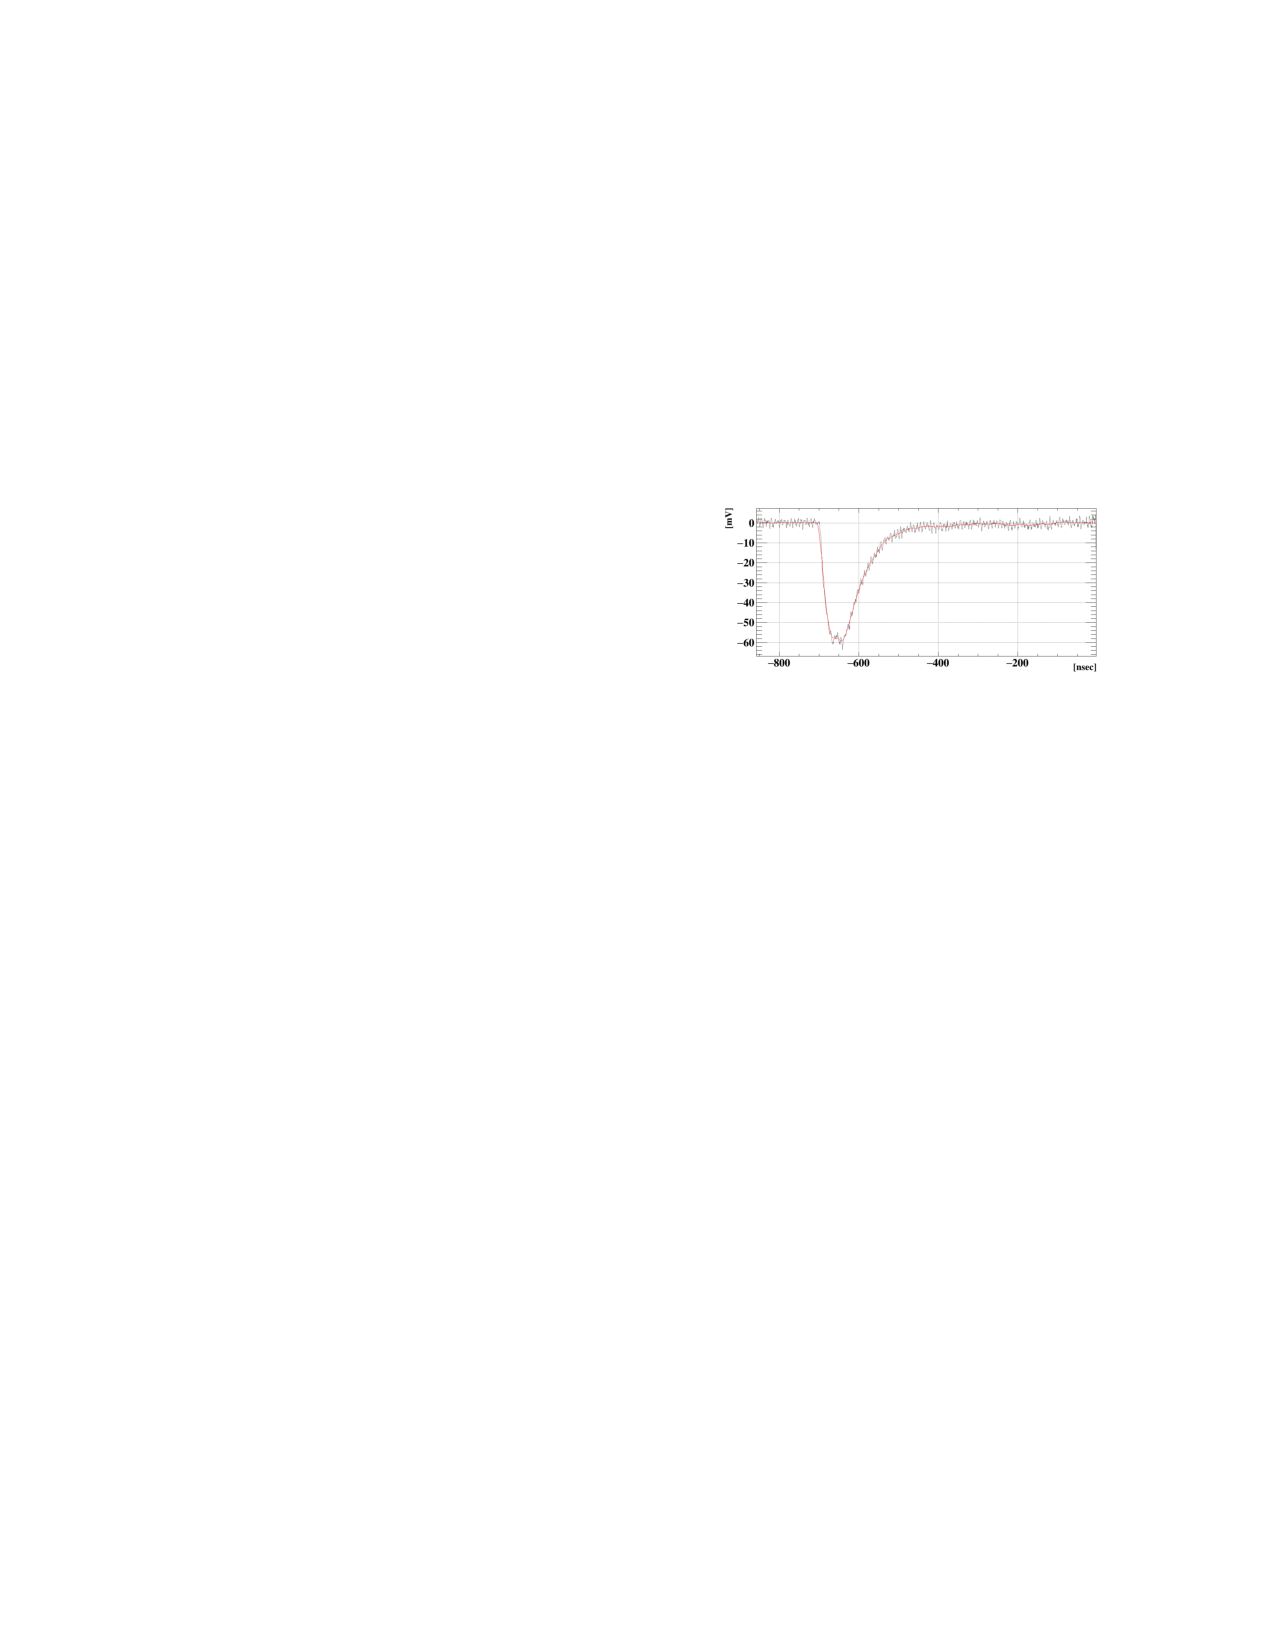
\includegraphics[scale=1.4]{figures/instruments/Waveform.pdf}
			\caption{Example Waveform recorded by DRS4}
		\end{figure}
	\begin{itemize}
		\item Select the \textcolor{blue}{channel} of interest (ch 0 $\longrightarrow$ 11)
		\item Measure the amplitude of the signal ($\pm$ 5 mV)
		\item Correlate with the \textcolor{red}{trigger value}  ($\pm$ 3 mV)
	\end{itemize}  
\end{frame}

%==================================================================
				%SLIDE 5 
%==================================================================
\begin{frame} [fragile]
\small
	\frametitle{Amplitude and Trigger correlation}
    		\begin{figure}
		 \centering
			\includegraphics[scale=0.3]{figures/instruments/Waveform_trigger.png}
			\caption{Example Waveform recorded by DRS4}
		\end{figure}  
	\begin{itemize}
		\item By changing the amplitude from a minimum value (300 mV) to a maximum value (full scale), in steps of 25 mV, \colorbox{yellow}{check the linearity} between the amplitude value and the trigger value.
	\end{itemize}
\end{frame}

%---------------------------------------------------------------------------------------------
%  RESULTS
%---------------------------------------------------------------------------------------------
	\section{Results}
		\subsection{Fits}
			%==================================================================
				%SLIDE
%==================================================================
\begin{frame} [fragile]
\small
	\frametitle{Channels calibration 0}
    		\begin{figure}
		 \centering
			\includegraphics[scale=0.5]{figures/ch0.pdf}
			%\caption{Channel 0.}
		\end{figure}  
\end{frame}

			%==================================================================
				%SLIDE
%==================================================================

\begin{frame} [fragile]
\small
	\frametitle{Channels calibration 1}
    		\begin{figure}
		 \centering
			\includegraphics[scale=0.5]{figures/ch1.pdf}
			%\caption{Channel 1.}
		\end{figure}  
\end{frame}

			%==================================================================
				%SLIDE
%==================================================================

\begin{frame} [fragile]
\small
	\frametitle{Channels calibration 2}
    		\begin{figure}
		 \centering
			\includegraphics[scale=0.5]{figures/ch2.pdf}
			%\caption{Channel 2.}
		\end{figure}  
\end{frame}

			%==================================================================
				%SLIDE
%==================================================================

\begin{frame} [fragile]
\small
	\frametitle{Channels calibration 3}
    		\begin{figure}
		 \centering
			\includegraphics[scale=0.5]{figures/ch3.pdf}
			%\caption{Channel 3.}
		\end{figure}  
\end{frame}
			%==================================================================
				%SLIDE
%==================================================================

\begin{frame} [fragile]
\small
	\frametitle{Channels calibration 4}
    		\begin{figure}
		 \centering
			\includegraphics[scale=0.5]{figures/ch4.pdf}
			%\caption{Channel 4.}
		\end{figure}  
\end{frame}
			%==================================================================
				%SLIDE
%==================================================================

\begin{frame} [fragile]
\small
	\frametitle{Channels calibration 5}
    		\begin{figure}
		 \centering
			\includegraphics[scale=0.5]{figures/ch5.pdf}
			%\caption{Channel 5.}
		\end{figure}  
\end{frame}

			%==================================================================
				%SLIDE
%==================================================================

\begin{frame} [fragile]
\small
	\frametitle{Channels calibration 6}
    		\begin{figure}
		 \centering
			\includegraphics[scale=0.5]{figures/ch6.pdf}
			%\caption{Channel 6.}
		\end{figure}  
\end{frame}

			%==================================================================
				%SLIDE
%==================================================================

\begin{frame} [fragile]
\small
	\frametitle{Channels calibration 7}
    		\begin{figure}
		 \centering
			\includegraphics[scale=0.5]{figures/ch7.pdf}
			%\caption{Channel 7.}
		\end{figure}  
\end{frame}
			%==================================================================
				%SLIDE
%==================================================================

\begin{frame} [fragile]
\small
	\frametitle{Channels calibration 8}
    		\begin{figure}
		 \centering
			\includegraphics[scale=0.5]{figures/ch8.pdf}
			%\caption{Channel 8.}
		\end{figure}  
\end{frame}
			%==================================================================
				%SLIDE
%==================================================================

\begin{frame} [fragile]
\small
	\frametitle{Channels calibration 9}
    		\begin{figure}
		 \centering
			\includegraphics[scale=0.5]{figures/ch9.pdf}
			%\caption{Channel 9.}
		\end{figure}  
\end{frame}
			%==================================================================
				%SLIDE
%==================================================================

\begin{frame} [fragile]
\small
	\frametitle{Channels calibration 10}
    		\begin{figure}
		 \centering
			\includegraphics[scale=0.5]{figures/ch10.pdf}
			%\caption{Channel 10.}
		\end{figure}  
\end{frame}
			%==================================================================
				%SLIDE
%==================================================================
\begin{frame} [fragile]
\small
	\frametitle{Channels calibration 11}
    		\begin{figure}
		 \centering
			\includegraphics[scale=0.5]{figures/ch11.pdf}
			%\caption{Channel 11.}
		\end{figure}  
\end{frame}

		\subsection{Table}
			%%==================================================================
				%SLIDE
%==================================================================
\begin{frame} [fragile]
\begin{equation*}
\text{Trigger value} =  a \times \text{DRS-Amplitude} + b
\end{equation*}

\begin{center}
\begin{tabular}{ ccc } 
 \hline
\textbf{Channel} & a  [$\text{mV}^{-1}$]& b [mV] \\ 
 \hline
 \hline
00 & 0.9255 $\pm$ 0.01877 & -7.373 $\pm$ 8.133 \\ 
01 & 0.9283 $\pm$ 0.01881 & -13.65 $\pm$ 8.151 \\
02 & 0.925   $\pm$ 0.01876 & -9.959 $\pm$ 8.13 \\
03 & 0.9199 $\pm$ 0.01869 & -12.5   $\pm$ 8.1 \\
04 & 0.9169 $\pm$ 0.01865 & -9.624 $\pm$ 8.084 \\
05 & 0.9262 $\pm$ 0.01879 & -16.15 $\pm$ 8.142 \\
06 &    0.92  $\pm$ 0.0187   & -7.043 $\pm$ 8.102 \\
07 & 0.9217 $\pm$ 0.01872 & -12.57 $\pm$ 8.112 \\
08 & 0.8958 $\pm$ 0.02114 & -3.705 $\pm$ 8.988 \\
09 & 0.9109 $\pm$ 0.01803 & -13.49 $\pm$ 7.848 \\
10 & 0.9003 $\pm$ 0.01788 & -5.758 $\pm$ 7.782 \\
11 & 0.904 $\pm$ 0.01815   & -7.483 $\pm$ 7.884 \\
  \hline
  \hline
\end{tabular}
\end{center}
The parameters are different because the \textit{chips}, that are on the gain lines of all the channels, are different.
\end{frame}

			\input{table_calibration2.tex}


%==================================================================
						%SLIDE - thebibliography
%==================================================================
%\begin{frame}
%\frametitle{\refname}
   \begin{thebibliography}{9}
   \small

      \bibitem{ROBERTO} Tesi di Laurea, Roberto Zarrella 2018-19
      \bibitem{MARCO} Tesi di Laurea, Marco Montefiori 2019-20
      %\newblock \textit{Thesis_Roberto_Zarrella}
      %\newblock \emph{Tesi di Laurea}, 2018-2019
   \end{thebibliography}
\end{frame}
%==================================================================

\end{document}